\section{Konzept}
\label{sec:TeilB_Konzept}
Um die Entwicklung zielführend zu gestalten ist neben der Bauteilrecherche eine grobe Hardwarearchitektur zu erstellen, welche sich im Laufe immer mehr verfeinert. Die letztendliche Architektur wird als Ausgangspunkt für weitere Entwicklungen genommen. Treten Probleme während der Entwicklung auf, wie z. B. Bauteile können nicht geliefert/sind zu teuer oder gewünschte Bauform so nicht verfügbar, sind Alternativen zu finden, mit dem Ziel das Konzept bestenfalls nur minimal ändern zu müssen. Um solchen Problem aus dem Weg zu gehen, ist eine vollständiges Konzept sowie eine Bauteildatenbank inklusive Lieferdaten der Bauteile im Vorfeld zu erstellen. Das Projekt orientiert sich bezüglich der Konversion von HDMI nach RGB und LVDS an der Application Note SLLA325A von Texas Instruments (siehe \cite{TI2011}).
\begin{figure}[htp]
%\begin{minipage}[t]{0.8\textwidth}
%\begin{figure}[h]
	\centering
\fbox{	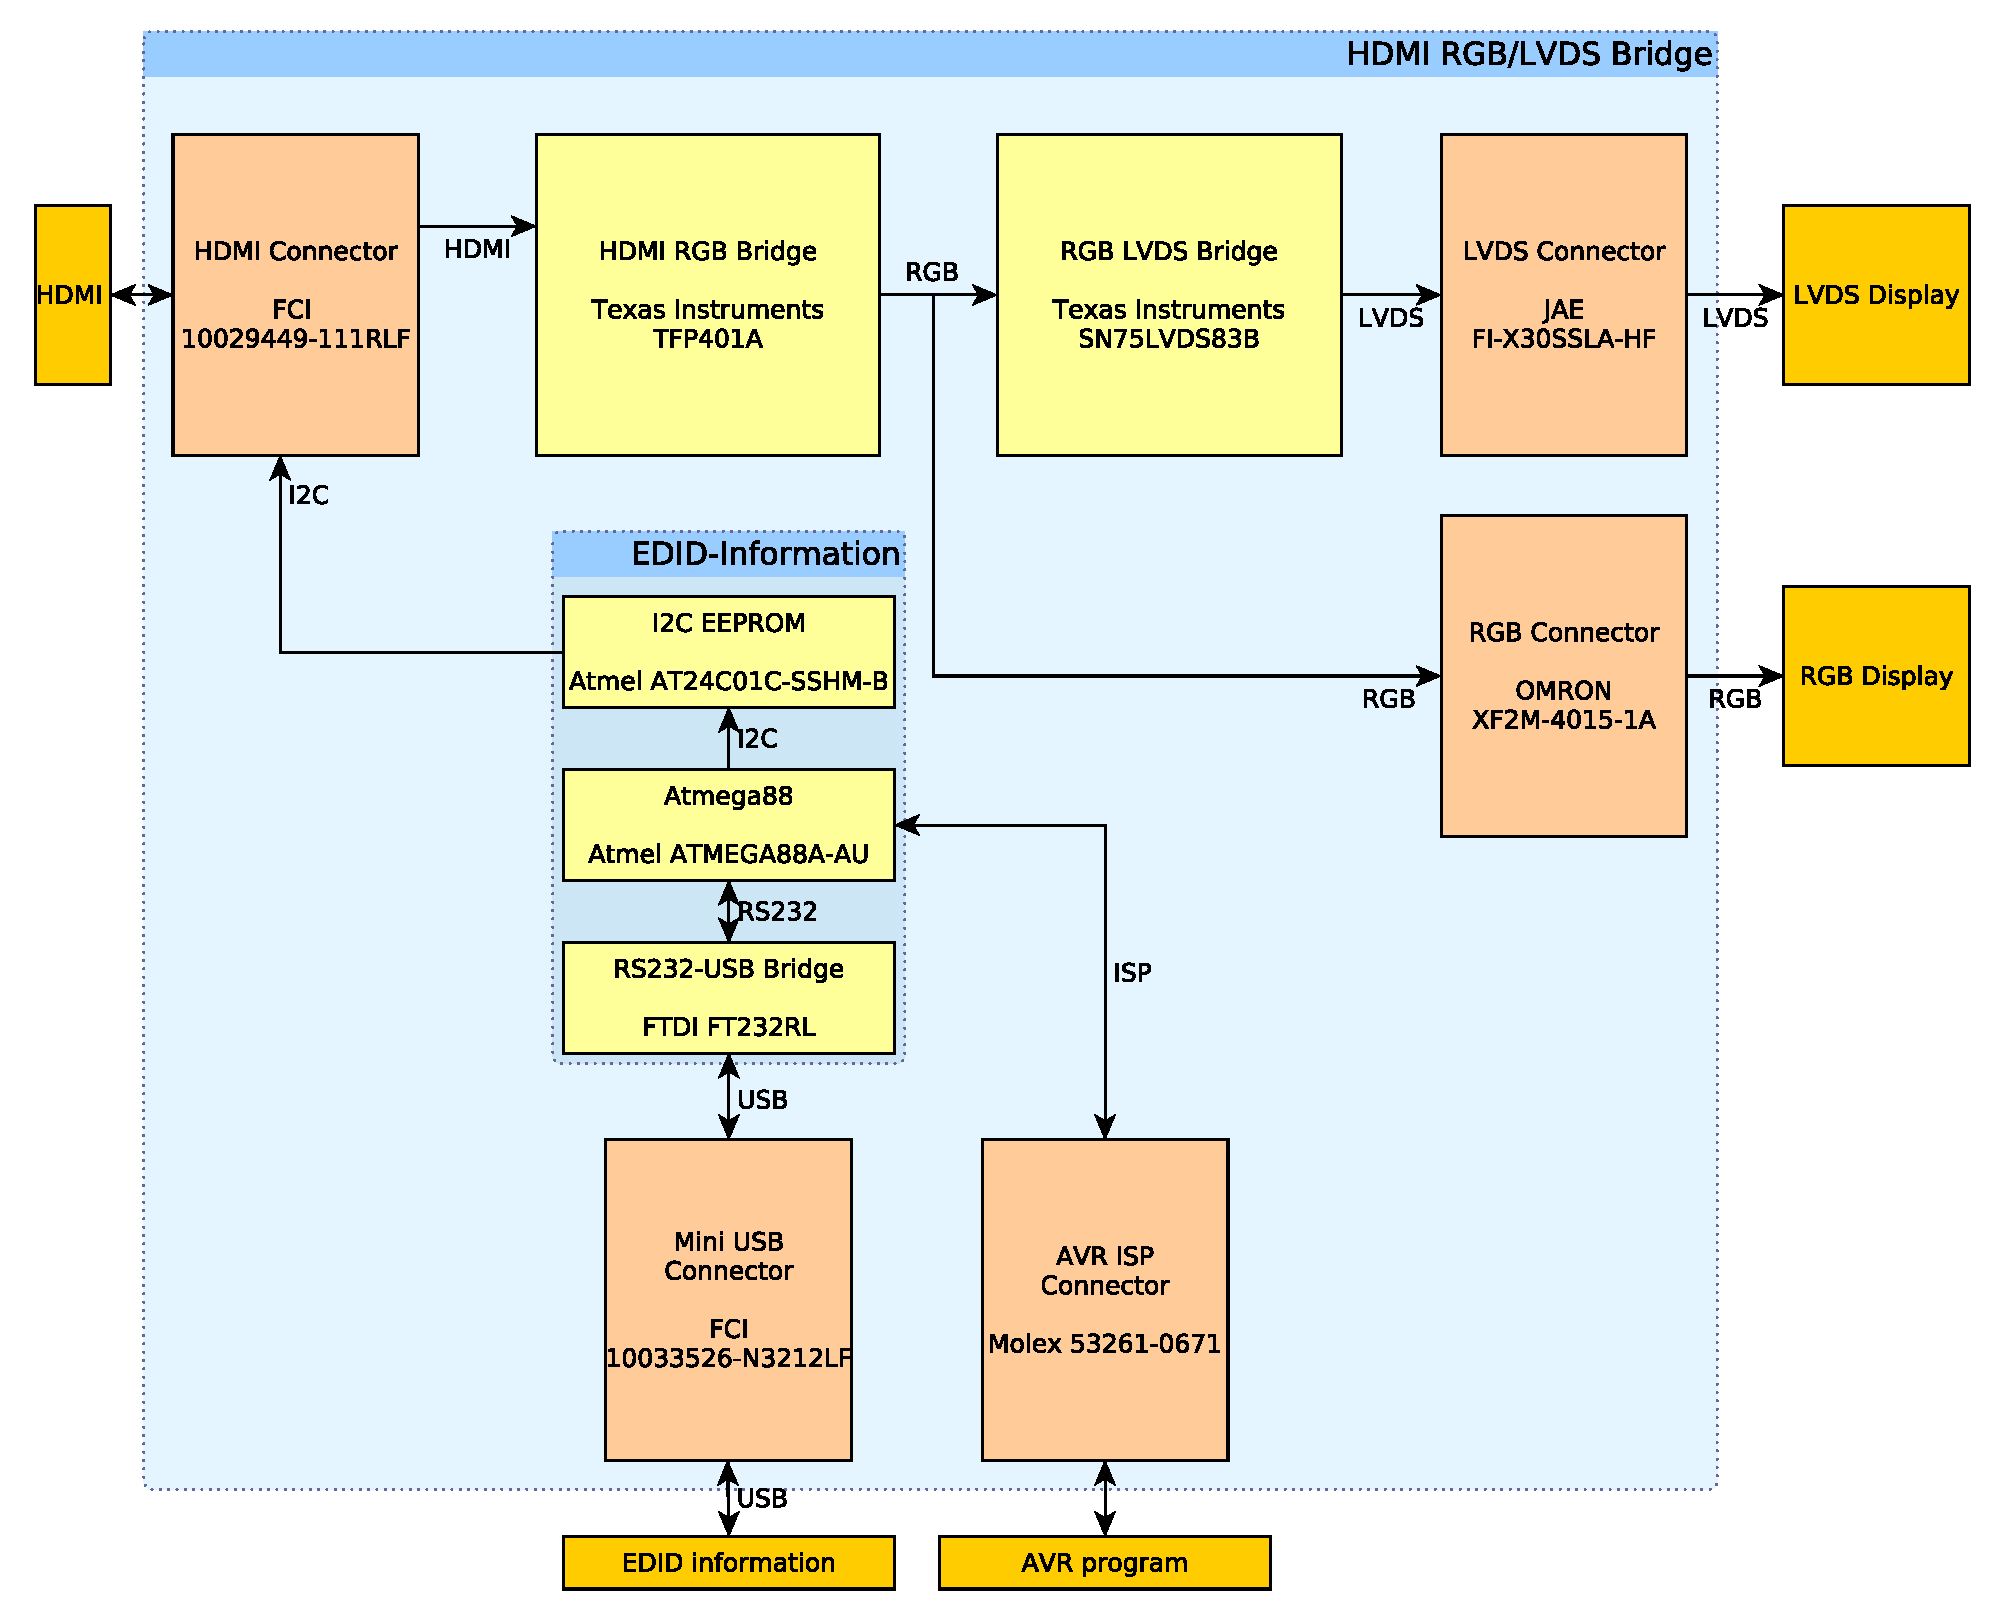
\includegraphics[width=1.0\textwidth]{TeilB/Architektur.pdf}}
	\caption{Teil B: Hardware-Architektur}
	\label{fig:teilb_architektur}
\end{figure}

\refa{fig:teilb_architektur} zeigt die komplette Architektur des Projekts mit allen, für das Projekt notwendigen Eckpunkten und Verbindungen. So sind Schnittstellen nach Assen mit Rot markiert und die interne Logik mit Gelb. Als Signalquelle wird das HDMI-Signal eingespeist und in die HDMI-RGB-Bridge geleitet. Der Baustein \code{TFP401A} konvertiert die eingehenden HDMI-Signale auf den RGB-Bus. Hier kann direkt über einen FPC-Stecker\footnote{FPC: Fine Pitch Connector} ein RGB-Display anschlossen werden. Die Leitungen werden weitergeleitet zu einer RGB-LVDS-Bridge. Diese wandelt die RGB-Signale in LVDS-Signale entsprechend der benötigten Beschaltung des verwendeten Displays um. Verbindet man die Platine mit einer HDMI-Quelle, so tauschen diese Informationen aus und der Monitor sendet seine Leistungsfähigkeit bzgl. Auflösung, Timings, etc. an die Quelle. Diese Daten werden als EDID-Daten\footnote{EDID: Extended Display Identification Data} bezeichnet (siehe )\todo{gute EDID quelle suchen!}. Gespeichert werden die EDID-Daten üblicherweise in einem EEPROM\footnote{EEPROM: Electrically Eraseable Programmable Read-Only Memory}, auf welches mit dem I2C-Bus zugegriffen werden kann. Um dieses EEPROM mit dem korrekten Inhalt beschreiben zu können, ist eine Baugruppe, in \refa{fig:teilb_architektur} mit EDID-Information markiert, realisiert, welche über die USB-Schnittstelle nutzbar ist. Der USB-Seriell-Konverter FT232RL kommuniziert mit einem 8 Bit Atmel ATMega88 Prozessor, welcher das I2C-EEPROM direkt beschreiben kann. Zur Kommunikation mit dem Prozessor und entsprechend dem EEPROM ist eine PC Software vorhanden, welche im Rahmen des Projekts entwickelt wurde (siehe \todo{Referenz auf PC Software}). \newpage